\section{Produkt"ubersicht}%

\textit{Worthwhile} ist ein m"achtiges Analysewerkzeug f"ur eine einfache WHILE-""Programmiersprache. Bei der Programmanalyse kommen dabei sowohl klassische Techniken der Laufzeitanalyse (interaktives Debuggen, Überprüfung von Zusicherungen zur Laufzeit) als auch moderne, logikbasierte Methoden der Softwareverifikation zum Einsatz.\footnote{Quelle: Projektspezifikation unter \url{http://formal.iti.kit.edu/teaching/pse/2011/}} \textit{Worthwhile} vereinigt s"amtliche Arbeitsschritte von der Programmerstellung bis zur Programmverifikation unter einer einzigen komfortablen und leicht benutzbaren Oberfl"ache. Außerdem ist \textit{Worthwhile} Ausführungsumgebung für die entwickelten WHILE-""Programme.%

\subsection{Anwendungsfall-""Übersicht}

Im folgenden Anwendungsfalldiagramm sind die unterschiedlichen Möglichkeiten zur Benutzung des Systems dargestellt:

\begin{figure}[H]
	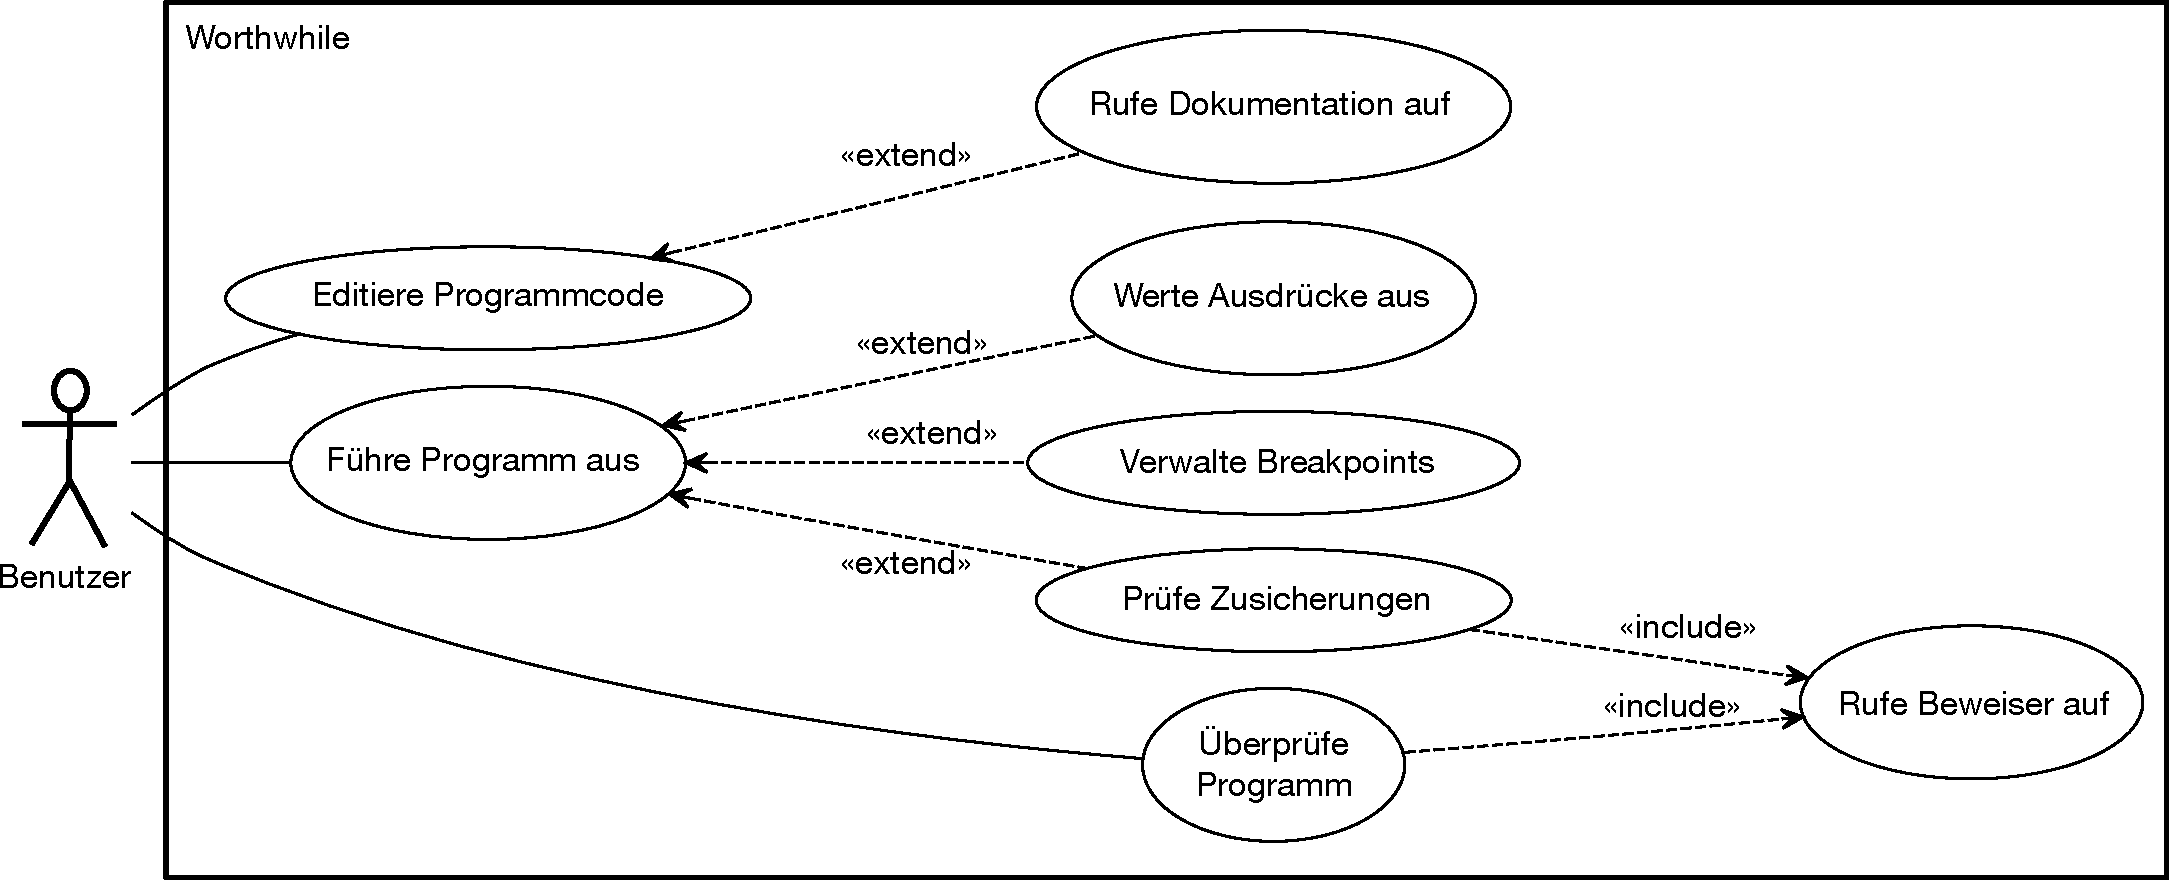
\includegraphics[width=\textwidth]{usecase/usecase.pdf}
\end{figure}

\subsubsection{Kurzbeschreibung der Anwendungsfälle}

Die einzelnen Anwendungsfälle umfassen jeweils die folgenden Tätigkeiten:

\begin{description}
	\item[Editiere Programmcode] Erstellen und Bearbeiten des Programmcodes unter Verwendung der GUI-Hilfsmittel wie Syntaxhervorhebung, Fehlerübersicht etc.
	\item[Rufe Dokumentation auf] Aufrufen der Dokumentation aus dem Programm heraus über einen GUI-Befehl oder eine kontextsensitive Hilfe.
	\item[Führe Programm aus] Ausführen oder Debuggen des Programms mit Hilfe des Interpreters; Ausführen im Einzelschrittmodus; Ausführen bis zum nächsten Breakpoint.
	\item[Werte Ausdrücke aus] Eingabe und Auswertung von benutzerdefinierten Ausdrücken über dem Programmzustand; Ändern von Variablenwerten im laufenden Programm.
	\item[Verwalte Breakpoints] Setzen und Löschen von Breakpoints; Festlegung von Bedingungen für Breakpoints.
	\item[Prüfe Zusicherungen] Überprüfen einzelner Zusicherungen im Programmtext zur Laufzeit mit Hilfe des Run-time-Checkers.
	\item[Überprüfe Programm] Statische Analyse des gesamten Programmes starten.
	\item[Rufe Beweiser auf] Externes Beweisermodul aus der GUI heraus aufrufen.
\end{description}